\section{From \mcms\ to \rts}\label{sec:rt-cons}

In this section, we provide a mapping from \mcms\ to \rts.
Specifically,
given an \mcm\ $CM_i$ that is specified through a set $S_{CM}$ of \synpats, we automatically infer a set of \rts, sufficient to enforce $CM_i$. 
In the rest of this section, we first differentiate between regular and irregular \synpats\ (\S\ref{sec:rt-cons:reg}). Then we provide the mapping (\S\ref{sec:rt-cons:map}), prove its correctness for an example \synpat\ (\S\ref{sec:rt-cons:pr}), extend the proof to all regular \synpats\ (\S\ref{sec:rt-cons:reg-ex}) and finally extend the proof to irregular \synpats\ (\S\ref{sec:rt-cons:irreg}).
In \tabref{tab:rt-sGLT}, we provide the mapping of 16 \synpats\ to \rts.
 
\subsection{Regular and irregular \synpats} \label{sec:rt-cons:reg}

We first categorize \synpats\ into two classes: \emph{regular} and \emph{irregular}.
A regular \synpat\ is 1) composed by alternating $\potype$ and $\syntype$ relations and 2) starts and ends on a $\potype$. Thus, any regular \synpat\ $s$, is of the following form:
\begin{equation*}
    s \triangleq \potype ; \syntype; \potype; ...\ \syntype; \potype
\end{equation*}
Any \synpat\ that does not conform to regularity rules is \emph{irregular}.
The distinction between regular and irregular \synpats\ will aid in the  presentation of the mapping from \synpats\ to \rts. Specifically, we will first create a mapping from a regular \synpat\ to the sufficient \rts\ to enforce it. Then, in order to use the same mapping for irregular \synpats, we will show that for every irregular \synpat\ $s_i$, there exists a regular \synpat\ $s_r$, such that enforcing $s_r$ is sufficient to enforce $s_i$. 


\subsection{The mapping} \label{sec:rt-cons:map}

We assert the following three conditions to enforce any regular \synpat, assuming that an operation can be of type $m$ or $n$ where $m, n \in$ $\{read, write\}$.
\squishlist
\item \emph{Cond-1}: for every $\potype$ relation $po_{mn}$ found in $s$, the corresponding \prt\ $prt_{mn}$ must be enforced. Plainly any $\potype$ relation must also be an $hb$ relation. 

\item \emph{Cond-2}: for every $\syntype$ relation $syn_{mn}$, if it is not an $rf$, then the \emph{reverse} \srt\ $srt_{nm}$ must be enforced. 

\item \emph{Cond-3}: if the first operation in $s$ is of type $m$ and the last of type $n$, the corresponding \srt\ $srt_{mn}$ must be enforced.

\squishend

\subsection{Proof for an example \synpat} \label{sec:rt-cons:pr}
We will start by first proving that the three conditions are sufficient for the simple \synpat, that is portrayed in \figref{fig:synpat}a. Then we will extend to any regular \synpat.
The simple \synpat\ $s$ is the following:
\begin{equation*}
    s \triangleq \powr ; fr ; \powr
\end{equation*}
For $s$ the three conditions require the following \rts:
\squishlist
\item \emph{Cond-1}: The $\prtwr$ is required for both $\powr$ relations.

\item \emph{Cond-2}: The $\rtwr$ for the $fr$ (\ie $\synrw$) relation.

\item \emph{Cond-3}: The $\rtwr$ because  $s$ starts with a write and ends on a read.
\squishend

\custvspace
We will show that for any execution \Exec, if $\prtwr$ is enforced and there exists $rl \in RL$ such that $\rtwr$ is enforced then for the $syn$ that is derived from that $rl$ it holds that $acyclic(s \cup syn)$.

To prove this, we first establish a new relation named \emph{begins-before-completes} ($bbc$). 
For two operations $a, b$ we assert that if $b$ does not complete before $a$ begins (\ie $(b, a) \notin hb$), then $a$ begins before $b$ completes (\ie $(a, b) \in bbc$).
We establish the following rule:
\begin{equation*}
 \forall a,d \in M\ s.t.\  (a, d) \in  (hb;bbc;hb) \rightarrow (a,d) \in hb
\end{equation*}
We sketch a proof for this rule using \figref{fig:bbc}a .
\figref{fig:bbc}a illustrates this through
four operations ($a,b,c,d$), each of which is associated with a timestamp ($ta$, $tb$, $tc$, $td$).
Operation $b$ begins before $c$ completes (\ie $(b,c)\in bbc$), while also $(a,b)$, $(c, d)$ $\in hb$. Therefore, $(a, d) \in (hb;bbc;hb)$.
Since $a$ completes before $b$ begins ($ta < tb$) and $b$ begins before $c$ completes ($tb < tc$), it follows that $a$ completes before $c$ completes ($ta < tc$). Because $c$ completes before $d$ begins ($tc < td$), it follows that $a$ completes before $d$ begins ($ta < td$). Therefore, $(a, d) \in hb$.

\figref{fig:bbc}b illustrates the counter-example, where $c$ completes before $b$ begins; in this case it is possible for $d$ to begin before $a$ completes.


\begin{figure}[t]
  \centering
  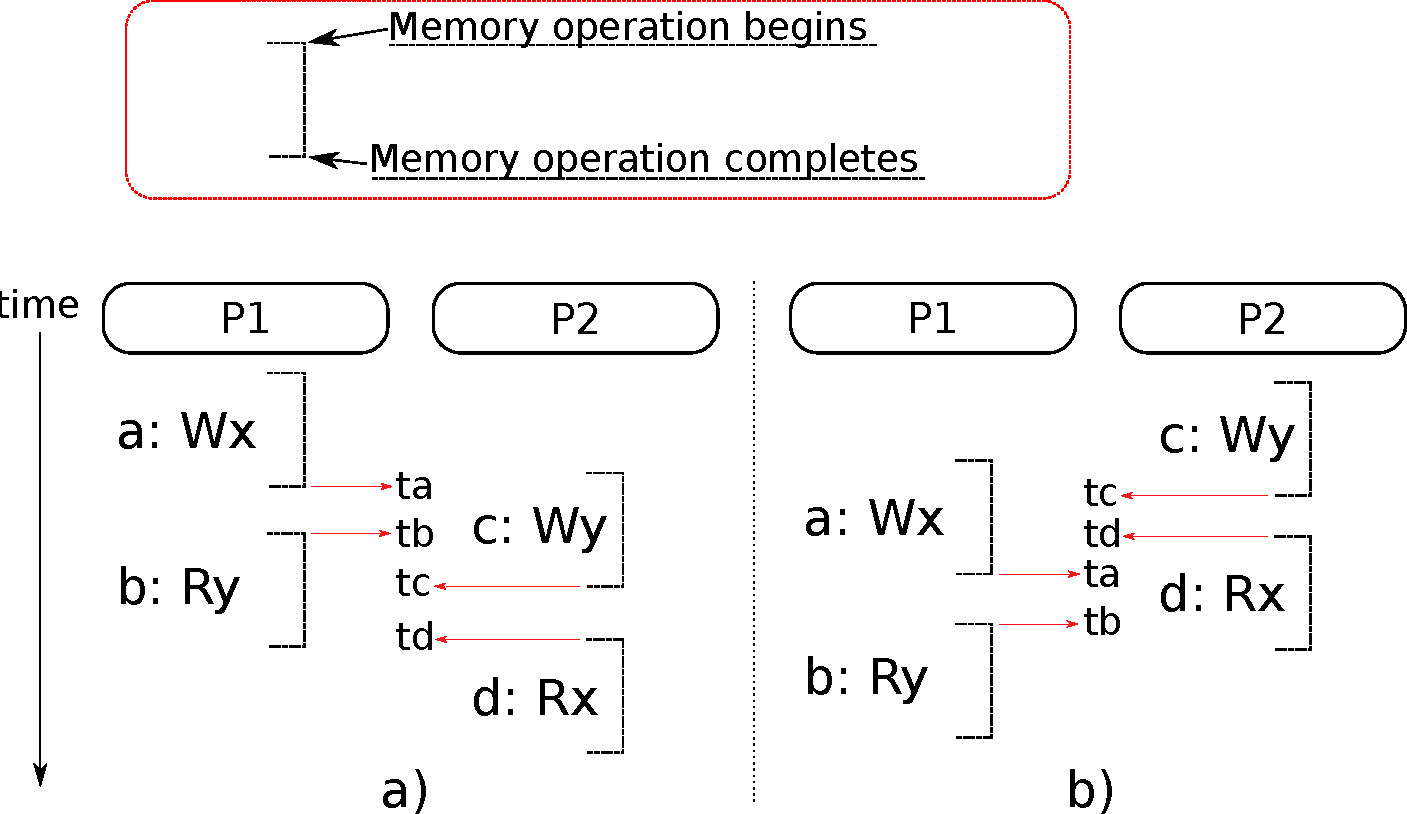
\includegraphics[width=0.35\textwidth]{1_figures/hb-bbc-hb.pdf}
  \caption{a) $b$ begins before $c$ completes  b) $c$ completes before $b$ begins. }
  \vspace{-1em}
  \label{fig:bbc}
\end{figure}


Consider an execution \Exec, for which there exists an $rl \in RL$ such that all three conditions we asserted are satisfied.
Assume four operations $a,b,c,d \in M$ such that $(a, b) \in \powr \andm (b,c) \in \synwr \andm (c,d) \in \powr$. This implies that $(a, d) \in s$.
Let us now assume that 
$(a, d) \in  (hb;bbc;hb)$ and thus $(a,d) \in hb$. Specifically, $(a,d) \in \hbwr$. This is illustrated in \figref{fig:bbc}a.
From the cond-3 ($\rtwr$), we can assert that since $(a,d) \in \hbwr$ it follows that $(d, a) \notin syn$ and thus it must be that $acyclic(s \cup syn)$.
Plainly, cond-3 ensures that  $acyclic(s \cup syn)$ if  the following condition holds: 
\begin{equation*}
 \forall a,d \in M\ s.t.\  (a, d) \in  s \rightarrow (a,d) \in hb
\end{equation*}
Therefore it suffices to prove that cond-1 and cond-2 guarantee the above condition. We will do so by proving that $(a, d) \in (hb;bbc;hb)$.

Firstly, cond-1 ($\prtwr$) mandates that $\powr \subseteq \hbwr$.
Therefore, $(a, b)$, $(c, d) \in hb$. 
We need only prove that $(b, c) \in bbc$. 
Let's assume that $(b, c) \notin bbc$. It follows that $(c, b) \in hb$.
Recall, that $b$ is a write and $c$ is a read. Cond-2 mandates that $\rtwr$ is enforced: since $(c, b) \in hb$ then $(b, c) \notin syn$. 
We have reached a contradiction, and therefore it must be that $(b, c) \in bbc$.

\figref{fig:bbc}b provides the counter example where $(b, c) \notin bbc$.
In this case it cannot be that $(a,d) \in s$ because $(b, c) \in hb$ and therefore from cond-2 it follows that $(c, b) \in syn$. Plainly, the \synpat\ $s$ will not occur here because P1's read to $y$ will observe P2's write to $y$.

As we have shown above, from cond-1 and cond-2 it follows that $(a, d) \in  hb$ and thus from cond-3 it follows that $(a, d) \notin syn$. Therefore the three conditions are sufficient to enforce $s$.

\subsection{Extending to all regular \synpats} \label{sec:rt-cons:reg-ex}
Note the intuition behind the three conditions. Cond-1 ensures that every $\potype$ relation of the \synpat\ is also an $hb$ relation. Similarly, cond-2 ensures that every $\syntype$ relation is also a $bbc$ relation. As a regular \synpat\ is composed by alternating $\potype$ and $\syntype$ relations, enforcing cond-1 and cond-2 ensures that the \synpat\ can be expressed as a composition of alternating $hb$ and $bbc$ relations.

As we saw $hb;bbc;hb \subseteq hb$. By induction we can extend this rule for any sequence of alternating $hb$ and $bbc$ relations. Specifically:
\begin{equation*}
\forall a,b \in M\ s.t.\ (a, b) \in hb;bbc;hb\ ....\ hb;bbc;hb \rightarrow (a,b) \in hb
\end{equation*}
Therefore, cond-1 and cond-2 ensure that if $(a, b) \in s$ then $(a,b) \in hb$ for any regular \synpat\ $s$. Finally, cond-3 ensures that the \synpat\ is enforced, by ensuring that if $(a,b) \in hb$ then $(b,a) \notin syn$.
This means that our three conditions can be used to enforce any regular \synpat.

\beginbsec{Examples -- \tabref{tab:rt-sGLT}}
\tabref{tab:rt-sGLT} depicts the sufficient \rts\ for 16 \synpats. Specifically, each cell represents a distinct \synpat\ between operations $a,b,c,d$. For instance, the highlighted cell where $a = Wx$, $b = Ry$, $c = Wy$, $d = Rx$, corresponds to the \synpat\ of \figref{fig:synpat}a.

\beginbsec{Cond-2 exception: $\mathbf{rf}$}
Recall that cond-2 is not required for $rf$ edges. This is because the purpose of cond-2 is to ensure that the $\syntype$ relation is also a $bbc$ relation. However, this is implied by the $rf$ as it is impossible for a read $r$ to read-from a write $w$ if $r$ completes before $w$ begins. Plainly: 
$\forall w,r \in M\ s.t.\  (w,r) \in rf \rightarrow (w,r) \in bbc $.
    
\beginbsec{Producer-consumer (\figref{fig:intro-ex}a)}
Let $s_{pc}$ be the producer-consumer \synpat\ of \figref{fig:intro-ex}a (discussed in the Introduction). We assert that $s_{pc} \triangleq \poww; rf;\porr$. To enforce $s_{pc}$, cond-1 requires \prts\ $\prtww, \prtrr$, cond-2 does not require any \srt\ because the only $\syntype$ is an $rf$ and cond-3 requires the $\rtwr$.




\begin{table}[t]
\centering
\footnotesize
 \resizebox{0.48\textwidth}{!}{%
\begin{tabular}{c|c|c|c|c|}
\hhline{~----}
                                                        
 & 
\headercell{c = Wy \\ d = Ry} &
\headercell{c = Wy\\ d = Wy} &
\headercell{c = Ry\\ d = Ry} &
\headercell{c = Ry\\ d = Wy}
\\ \hline
\multicolumn{1}{|c|}{
\headercell{a = Wx\\ b = Rx}} & 
\cellcolor[HTML]{9AFF99}  \itcell{$\rtwr$, \\ $\prtwr$}&
\itcell{$\rtww$, $\rtwr$, \\ $\prtwr$, $\prtww$}  &
\itcell{$\rtwr$,  $\rtrr$, \\ $\prtwr$, $\prtrr$}  & 
\itcell{$\rtww$,  $\rtrr$, \\ $\prtwr$, $\prtrw$}                                                         
\\ \hline
\multicolumn{1}{|c|}{
\headercell{a = Wx\\ b = Wx}} & 

\itcell{$\rtwr$, $\rtww$, \\$\prtww$, $\prtwr$}&
\itcell{$\rtww$, \\$\prtww$}  &
\itcell{$\rtwr$,  $\rtrw$, \\$\prtww$, $\prtrr$}  & 
\itcell{$\rtww$,  $\rtrw$, \\$\prtww$, $\prtrw$}  
\\ \hline
\multicolumn{1}{|c|}{
\headercell{a = Rx\\ b = Rx}} &

\itcell{$\rtrr$, $\rtwr$, \\ $\prtrr$, $\prtwr$}&
\itcell{$\rtrw$, , $\rtwr$, \\ $\prtrr$, $\prtww$}  &
\itcell{$\rtrr$, \\ $\prtrr$}  & 
\itcell{$\rtrw$,  $\rtrr$, \\ $\prtrr$, $\prtrw$}  
\\ \hline
\multicolumn{1}{|c|}{
\headercell{a = Rx\\ b = Wx}} &
\itcell{$\rtrr$, $\rtww$, \\ $\prtrw$, $\prtwr$}&
\itcell{$\rtrw$, , $\rtww$, \\ $\prtrw$, $\prtww$}  &
\itcell{$\rtrr$ ,  $\rtrw$, \\ $\prtrw$, $\prtrr$}  & 
\itcell{$\rtrw$, \\ $\prtrw$}  
\\ \hline
\end{tabular}%
}
\caption{The mapping of 16 \synpats\ to \rts. Each cell represents a \synpat\ of the form $s \triangleq \potype ; \syntype; \potype$, where the first $\potype$ includes $(a,b)$, the $\syntype$ includes $(b,c)$ and the second $\potype$ includes $(c,d)$. The highlighted cell corresponds to \figref{fig:synpat}a.}%
 \vspace{-1em}
\label{tab:rt-sGLT}
\end{table}

\subsection{Extending to irregular \synpats}\label{sec:rt-cons:irreg}

A \synpat\ is deemed \emph{irregular} if 1) it has consecutive $\potype$ relations or 2) it has consecutive $\syntype$ relations or 3) it does not start with a $\potype$ relation (\ie starts with $\syntype$) or 4) it does not end with a $\potype$ relation (\ie ends with $\syntype$).
For each such \synpat\ $s$, we derive a \synpat\ $s'$ such that 1) $s'$ is regular and 2) if $s'$ is enforced then $s$ must also be enforced.



\beginbsec{Consecutive po-type}
We start with \synpats\ with consecutive $\potype$ relations.
We use the insight that any composition of $\potype$ relations must be the subset of one of $\poww$, $\powr$, $\porr$, $\porw$ relation. 
For instance $\poww;\powr;\porr;\porw$ is a subset of $\poww$. Therefore, for any $s$ that has consecutive composed $\potype$ relations, we derive a $s'$ which replaces them with a single $\potype$ relation, such that $s \subseteq s'$ and we assert that enforcing $s'$ is sufficient to also enforce $s$. Below is an example of $s$ and the derived $s'$ using the insight that 
$(\powr ; \porw) \subseteq \poww$.
\begin{gather*}
    s \triangleq \powr ; \porw; \synwr; \porr \\
    s' \triangleq \poww; \synwr; \porr
\end{gather*}



Note that an alternative approach would have been to omit deriving $s'$ and instead simply asserting that the first condition is applied for each $\potype$ relation in $s$. That would still be correct and can be used.

\beginbsec{Consecutive syn-type}
Our approach is identical for \synpats\ with consecutive composed $\syntype$ relations. Specifically, a composition of $\syntype$ relations is always a subset of one of $fr$, $ws$, $\synwr$, $\synrw$. This is because 
any pair in a composition of $\syntype$ relations is also in $syn$ and thus it must be in one of $fr, ws, \synwr \synrw$, as $syn$ is the union of these four relations.
Therefore, for any $s$ that has consecutive composed $\syntype$ relations, we derive an $s'$ which replaces them with a single $\syntype$ relation, such that $s \subseteq s'$.

\beginbsec{Begin with syn-type}
When a \synpat\ $s$ begins with a $\syntype$ relation, then we derive $s'$ by simply removing it.
Let us see why through an example.
Assume the following $s$ which starts with an $fr$ and the derived $s'$ which removes the $fr$:
\begin{gather*}
    s\triangleq fr ; \powr fr; \powr \\
    s' \triangleq\powr fr; \powr
\end{gather*}
Assume now that $(a,c) \in s$,  $(b,c) \in s'$ and $(a, b) \in fr$.
Let us now prove that if $s'$ is enforced, $s$ is enforced too.
Assume $s'$ is enforced but $s$ is not. Therefore, $(c,b) \notin syn$ but $(c, a) \in syn$. We know that $(a, b) \in fr$ and thus $(a, b) \in syn$. By the transitivity property of $syn$ we assert that since $(c, a) \in syn \andm (a, b) \in syn$ it must be that $(c, b) \in syn$. This contradicts our assumption that $s'$ is enforced.
Therefore enforcing $s'$ is sufficient to also enforce $s$.

\beginbsec{End on syn-type}
Similarly, if $s$ ends on a $\syntype$ relation, we remove it to derive $s'$.
Assume the following example.
\begin{gather*}
    s\triangleq \powr fr; \powr fr\\
    s' \triangleq\powr fr; \powr
\end{gather*}
Assume now that $(a,c) \in s$,  $(a,b) \in s'$ and $(b, c) \in fr$.
Using the same proof as above, we can infer that if $s'$ is enforced then $(b,a) \notin syn$ and thus it follows that $(c, a) \notin syn$. Therefore enforcing $s'$ is sufficient to also enforce $s$.

\beginbsec{A combination of the above (IRIW -- \figref{fig:intro-ex}b)}
When a \synpat\ falls into more than one of the above irregular categories, we combine the techniques discussed above. For instance, let $s_{iriw}$ be the IRIW \synpat\ of \figref{fig:intro-ex}b (discussed in the Introduction). 
\begin{equation*}
    s_{iriw} \triangleq rf;\porr;fr;rf;\porr
\end{equation*}
This is an irregular \synpat, which both starts with a $\syntype$ and includes a composition of consecutive $\syntype$ relations. We use the rules above to derive $s_{iriw}'\triangleq \porr;\synrr\porr$ and assert that if $s_{iriw}'$ is enforced then $s_{iriw}$ is also enforced.
To enforce $s_{iriw}'$, cond-1 requires the \prt\ $\prtrr$ and cond-2 requires the \srt\ $\rtrr$ which is also required by cond-3.











